\documentclass[a4paper, 11pt]{exam}
\usepackage[T1]{fontenc}
\usepackage{titling}
\usepackage{url}
\usepackage{amsmath,amsthm,amssymb}
\usepackage{graphicx}
\usepackage{graphics}
\usepackage{listings}
\usepackage[dvipsnames]{xcolor}
\usepackage{tabularx}
\usepackage{ragged2e}
\usepackage{courier}
\usepackage{textcomp}
\usepackage{circuitikz}
\usepackage{tikz}
\usepackage{enumitem}
\usepackage{karnaugh-map}
\usepackage{bytefield}
\usepackage{mathrsfs}
\usepackage{cancel}
\usepackage[linesnumbered,ruled,vlined]{algorithm2e}
\usepackage{hyperref}
\newcommand{\invlaplace}[1]{%
\mathscr{L}^{-1}\left\{#1\right\}
}
\newcommand{\laplace}[1]{%
\mathscr{L}\left\{#1\right\}
}
\newcommand{\fourier}[1]{%
\mathscr{F}\left\{#1\right\}
}

\newcommand{\ztransform}[1]{%
\mathscr{Z}\left\{#1\right\}
}

\newcommand{\subtitle}[1]{%
  \posttitle{%
    \par\end{center}
    \begin{center}\large#1\end{center}
    }%
}

\usepackage{environ}

\NewEnviron{eqnsection}[2]{%
  \newcommand{\myvspace}{#1}%
  \vspace{\myvspace}%
  \begin{align*}
  \intertext{#2}
  \BODY
  \end{align*}%
  \vspace{\myvspace}%
}


\newcommand{\uparrowat}[1]{\underset{\uparrow}{#1}}


\newlist{myenumerate}{enumerate}{2}
\setlist[myenumerate,1]{label=\roman*)}
\setlist[myenumerate,2]{label=\alph*)}



\newcommand\tab[1][1cm]{\hspace*{#1}}

\renewcommand{\labelenumi}{\alph{enumi})}

\title{Homework Assignment \#2}
\subtitle{ECE 6530: Digital Signal Processing \\
\today\\}
\author{ Miguel Gomez U1318856\\
\textbf{Homework set \#2}}
\date{Due Date: Sep 14, 2023\\
(100 points)}

\begin{document}
\maketitle
\noindent
\section{}
2.7 - Answer subquestions (1) through (5) for parts (a) through (e). (10 points)
\vspace{2em}
\hrule
\begin{enumerate}
\item $y(n) = \cos{(x(n))}$
\item $y(n) = \sum_{k=-\infty}^{n+1} x(k)$
\item $y(n) = x(n)\cos{(\omega_0n)}$
\item $y(n) = x(-n + 2)$
\item $y(n) = $Trun$[x(n)]$ where Trun$[x(n)]$ denotes the integer part of $x(n)$, obtained
by \\ truncation.
\end{enumerate}
\newpage
\section{}
2.11 - Problem 2.11 (10 points)
\begin{eqnsection}{3em}{The following input–output pairs have been observed during the operation of a linear system:}
  x_1 (n) &= \lbrace-1, \uparrowat{2}, 1\rbrace \quad \overset{\text{$\mathcal{T}$}}{\longleftrightarrow}\quad y_1(n)=\lbrace1,\uparrowat{2},-1,0,1\rbrace \\
  x_2 (n) &= \lbrace−1, \uparrowat{-1}, -1\rbrace \quad \overset{\text{$\mathcal{T}$}}{\longleftrightarrow}\quad y_2(n)=\lbrace-1,\uparrowat{1},0,2\rbrace \\
  x_3 (n) &= \lbrace0, \uparrowat{1}, 1\rbrace \quad \overset{\text{$\mathcal{T}$}}{\longleftrightarrow}\quad y_3(n)=\lbrace\uparrowat{1},2,1\rbrace \\
 \end{eqnsection}
 \newpage
 \begin{eqnsection}{0em}{Can you draw any conclusions about the time invariance of this system?}
   x_1 (n) + x_2 (n) &=  \lbrace-1, \textcolor{red}{\uparrowat{2}}, 1\rbrace + \lbrace−1, \textcolor{blue}{\uparrowat{-1}}, -1\rbrace\\
   y_1 (n) + y_2 (n) &= \lbrace1,\textcolor{red}{\uparrowat{2}},-1,0,1\rbrace + \lbrace-1,\textcolor{blue}{\uparrowat{1}},0,2\rbrace \\
   \intertext{Since the red match, we would expect the blue to match as well if they are time invariant. Since they do not, it tells us there is some relationship other than the impulse going on.}
 \end{eqnsection}
\hrule
\section{} 
2.16 - Problem 2.16 part (b3) and (b11) (10 points)
\newline
\begin{enumerate}
\item If $y(n) = x(n) \ast h(n)$, show that $\sum_y = \sum_x\sum_h$, where $\sum_x = \sum_{-\infty}^{\infty}x(n)$.
\item Compute the convolution $y(n) = x(n) \ast h(n)$ of the following signals and check the \\ correctness of the results by using the test in ($a$).
\end{enumerate}

\begin{enumerate}
  \item  [b3   )] $x(n) = \left\lbrace0, 1, -2, 3, -4\right\rbrace$, $ h(n) = \left\lbrace \frac{1}{2} , \frac{1}{2} , 1, \frac{1}{2} \right\rbrace$
  \item  [b11)] $x(n) =\left(\frac{1}{2}\right)^n u(n)$, $ h(n) =\left( \frac{1}{4}\right)^n u(n)$
\end{enumerate}
\hrule
\vspace{1em}
b3) Convolution of discrete systems can be done by matrix multiplication:
\begin{center}
\[
\begin{bmatrix}
x[0]&0&0&0\\
x[1]&x[0]&0&0\\
x[2]&x[1]&x[0]&0\\
x[3]&x[2]&x[1]&x[0]\\
x[4]&x[3]&x[2]&x[1]\\
0&x[4]&x[3]&x[2]\\
0&0&x[4]&x[3]\\
0&0&0&x[4]\\

\end{bmatrix} 
\cdot
\begin{bmatrix}
h[0]\\
h[1]\\
h[2]\\
h[3]
\end{bmatrix}
=
\begin{bmatrix}
y[0]\\
y[1]\\
y[2]\\
y[3]\\
y[4]\\
y[5]\\
y[6]\\
y[7]\\
\end{bmatrix}
\]
\end{center}
\begin{center}
\[
\begin{bmatrix}
0&0&0&0\\
1&0&0&0\\
-2&1&0&0\\
3&-2&1&0\\
-4&3&-2&1\\
0&-4&3&-2\\
0&0&-4&3\\
0&0&0&-4\\

\end{bmatrix} 
\cdot
\frac{1}{2}\begin{bmatrix}
1\\
1\\
2\\
1
\end{bmatrix}
=
\frac{1}{2}
\begin{bmatrix}
0\\
1\\
-2 + 1\\
3 -2 + 2\\
-4 + 3 - 4 + 1\\
-4 + 6 - 2\\
-8 + 3\\
-4\\
\end{bmatrix}
=
\frac{1}{2}
\begin{bmatrix}
0\\
1\\
-1\\
3\\
-4\\
0\\
-5\\
-4\\
\end{bmatrix}
=
\begin{bmatrix}
0\\
\frac{1}{2}
\\
-\frac{1}{2}
\\
\frac{3}{2}\\
-2\\
0\\
-\frac{5}{2}\\
-2\\
\end{bmatrix}
\]
\end{center}
\begin{center}
$y = \lbrace0,\frac{1}{2},-\frac{1}{2},\frac{3}{2},-2,0,-\frac{5}{2},-2 \rbrace$
\end{center}
\newpage
\vspace{1em}
\begin{eqnsection}{1em}{b11) can be done by expressing it as a sum:}
  x(n) &= \left(\frac{1}{2}\right)^n u(n)\text{,}\  h(n) =\left(\frac{1}{4}\right)^n u(n)\\
  x\ast h &= \sum_{k=-\infty}^{\infty}x(n)h(n-k)\ = \sum_{k=-\infty}^{\infty}h(k)x(n-k)\\
    \intertext{Swapping the order of the convolution should not make a difference}
    &= \sum_{k=-\infty}^{\infty}h(k)x(n-k) = \sum_{k=-\infty}^{\infty}\left(\frac{1}{4}\right)^k u(k)\left(\frac{1}{2}\right)^{(n-k)}u(n-k)\\
    \intertext{Since the sum goes from $k$ and is bounded by $n$, we can absorb those into the sum:}
    &= \sum_{k=0}^{n}\left(\frac{1}{4}\right)^k\left(\frac{1}{2}\right)^{(n-k)} = \sum_{k=0}^{n}\left(\left(\frac{1}{2}\right)^2\right)^k\left(\frac{1}{2}\right)^{(n-k)}\\
    &= \sum_{k=0}^{n}\left(\frac{1}{2}\right)^{2k}\left(\frac{1}{2}\right)^{-k}\left(\frac{1}{2}\right)^{n} = \sum_{k=0}^{n}\left(\frac{1}{2}\right)^{n+k}\\
    &= \left(\frac{1}{2}\right)^{n}\sum_{k=0}^{n}\left(\frac{1}{2}\right)^{k}\\
    \intertext{By the expression for a finite sum:}
    &= \sum_{k=1}^{n} = a\frac{1-r^n}{1-r}\ \ \& \quad r = \frac{1}{2}\\
    &=\left(\frac{1}{2}\right)^{n}a\frac{1-\left(\frac{1}{2}\right)^n}{1-\left(\frac{1}{2}\right)}\\
    &=a\frac{\left(\frac{1}{2}\right)^{n}-\left(\frac{1}{2}\right)^{n}\left(\frac{1}{2}\right)^n}{\left(\frac{1}{2}\right)}\\
    &=2a\left(\left(\frac{1}{2}\right)^{n}-\left(\frac{1}{2}\right)^{2n}\right)\\
    &=a\left(\left(\frac{1}{2}\right)^{n-1}-\left(\frac{1}{2}\right)^{2n-1}\right)\\
    &=a\left(\left(\frac{1}{2}\right)^{n-1}-\left(\frac{1}{2}\right)^{2n-1}\right)\\
    \left(\frac{1}{2}\right)^{n}\sum_{k=0}^{n}\left(\frac{1}{2}\right)^{k} &= \frac{a}{2}\left(2\left(\frac{1}{2}\right)^{n}-2\left(\frac{1}{2}\right)^{2n}\right)\\
    \left(\frac{1}{2}\right)^{n}\sum_{k=0}^{n}\left(\frac{1}{2}\right)^{k} &= a\left(\left(\frac{1}{2}\right)^{n}-\left(\frac{1}{4}\right)^{n}\right)\\
    \intertext{This started at $k = 0$ when the sum should start at 1 to be equal to the sum at the top. so the term for $a$ is just 1.}
    &= \left(\left(\frac{1}{2}\right)^{n}-\left(\frac{1}{4}\right)^{n}\right)u(n)
  \end{eqnsection}
  It seems that there is a factor of two missing in my work since the expression should have another 2 on the first term. Essentially making that term have an $n - 1$ in the exponent. Perhaps because the finite sum formula begins at 1 instead and ours begins at 0?
\begin{eqnsection}{0em}{verifying b3 with sums from a:}
  \sum_y = \sum_x\sum_h \quad\text{, where }  \quad \sum_x &= \sum_{-\infty}^{\infty}x(n) \\
  x(n) &= \left\lbrace0, 1, -2, 3, -4\right\rbrace\ \text{, } h(n) = \left\lbrace \frac{1}{2} , \frac{1}{2} , 1, \frac{1}{2} \right\rbrace \\
  \sum_x &= \sum\left\lbrace0, 1, -2, 3, -4\right\rbrace = -2 \\
  \sum_h &= \sum\left\lbrace \frac{1}{2} , \frac{1}{2} , 1, \frac{1}{2} \right\rbrace = \frac{5}{2} \\
  \sum_y = \sum_x\sum_h = \frac{5}{2} \cdot (-2) &= -5\\
  \sum_y = \sum\lbrace0,\frac{1}{2},-\frac{1}{2},\frac{3}{2},-2,0,-\frac{5}{2},-2 \rbrace &= -5 \\
\end{eqnsection}
\begin{eqnsection}{-2em}{Verifying b11 using $\sum_y = \sum_x\sum_h$, where $\sum_x = \sum_{-\infty}^{\infty}x(n)$}
  \sum_y = \sum_x\sum_h \quad\text{, where }  \quad \sum_x = \sum_{-\infty}^{\infty}x(n) \\
\end{eqnsection}
\newpage
\section{}
2.24 - Problem 2.24. (10 points)\\
\begin{eqnsection}{-2em}{The discrete-time system:}
  y(n) = ny(n - 1) + x(n)\text{,}\quad&\ \ \ n \ge 0
    \intertext{:is at rest [i.e., $y(−1) = 0$]. Check if the system is linear time invariant and BIBO stable.}
    y_1(n) + y_2(n) = ny_1(n - 1) &+ x_1(n) +  ny_2(n - 1) + x_2(n) \\
    y_1(n) + y_2(n) = ny_1(n - 1) +  ny_2(n - 1) &+ x_1(n) + x_2(n) \\
    y_1(n) + y_2(n) = n(y_1(n - 1) +  y_2(n - 1)) &+ (x_1(n) + x_2(n)) \\
    \intertext{$\therefore $ system is linear:}
    x(n-1) \rightarrow{} y(n-1) &= (n-1)y(n-1 -1) + x(n-1)\\
    n' &= n-1\\
    x(n-1) \rightarrow{} y(n-1) &= n'y(n'-1) + x(n')\\
    \intertext{$\therefore $ system is time-invariant. Giving the following is a bounded input:}
    x(n) &= u(n) \leq 1 \quad \forall n \geq 0\\
    \intertext{The following should be bounded as well:}
   y(1) &=  (1)y(0) + 1\\
   y(0) &=  -1\\
   y(2) &=  0 + 1\\
   y(3) &= 3y(2) + 1 = 4\\
   \intertext{This continues to increase and $\therefore $ it is unbounded.}
  \end{eqnsection}
\vspace{2em}
\hrule
\section{}
2.27 - Problem 2.27. Determine the homogeneous, particular and total solutions. (15 points)\\
\begin{eqnsection}{-1em}{Determine the particular solution of the difference equation:}
  y(n) = \frac{5}{6}y(n-1)-\frac{1}{6}y(n-2) + x(n)\\
  \intertext{when the forcing function is $x(n) = 2 u(n)$.}
\end{eqnsection}
\newpage
\begin{eqnsection}{0em}{}
  y_h(n) &= \lambda^nu(n)\\
  \lambda^{n} &= \frac{5}{6}\lambda^{n-1}-\frac{1}{6}\lambda^{n-1}\\
  \lambda^{n} -\frac{5}{6}\lambda^{n-1}+\frac{1}{6}\lambda^{n-2}&= 0\\
  \lambda^{2}\lambda^{n-2} -\frac{5}{6}\lambda^{n-2}\lambda+\frac{1}{6}\lambda^{n-2}&= 0\\
  \lambda^{n-2}\left(\lambda^{2} -\frac{5}{6}\lambda+\frac{1}{6}\right) &= 0\\
  \lambda^{2} -\frac{5}{2\ 3}\lambda+\frac{1}{2\ 3} &= 0 \\
  \left(\lambda - \frac{1}{2}\right)\left(\lambda - \frac{1}{3}\right) &= 0\\
\end{eqnsection}
\[
  r = 
\begin{bmatrix}
\frac{1}{2}&\frac{1}{3}\\
\end{bmatrix}  
\]
\vspace{2em}
\hrule
\section{}
2.31 - Problem 2.31. (10 points)\\
\begin{eqnsection}{-3em}{Determine the impulse response of the following causal system:}
  y(n) - 3y(n - 1) - 4y(n - 2) = x(n) + 2x(n - 1)
\end{eqnsection}
\vspace{2em}
\hrule
\section{}
2.46 - Problem 2.46. (10 points)\\
\begin{eqnsection}{-3em}{Determine the direct form II realization for each of the following LTI systems:}
  &\text{a) } 2y(n) + y(n - 1) - 4y(n - 3) = x(n) + 3x(n - 5)\\
  &\text{b) } y(n) = x(n) - x(n - 1) + 2x(n - 2) - 3x(n - 4)
\end{eqnsection}
\vspace{2em}
\hrule
\section{}
2.49 - Problem 2.49 part (a). Assume that the system is relaxed. (10 points)\\
A discrete-time system is realized by the structure shown in Fig. P49.\\
\begin{enumerate}
\item Determine the impulse response.
\item Determine a realization for its inverse system, that is, the system which produces $x(n)$ as an output when $y(n)$ is used as an input.
\end{enumerate}
\begin{figure}[ht!]
  \centering
  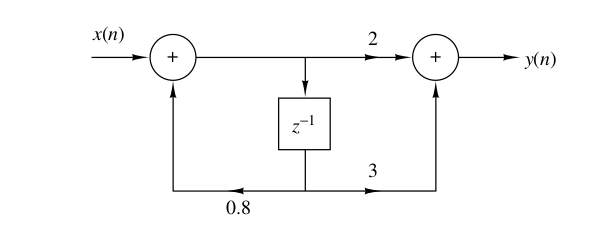
\includegraphics[width=10cm]{figures/fig49.png}
  \caption{Figure P49 from textbook}
    \label{fig:number49_fromText}
\end{figure}
\vspace{2em}
\hrule
\newpage
\section{}
2.52 - Problem 2.52 part (a). (15 points)\\
Consider the systems shown in Fig. P52.\\
\begin{figure}[ht!]
  \centering
  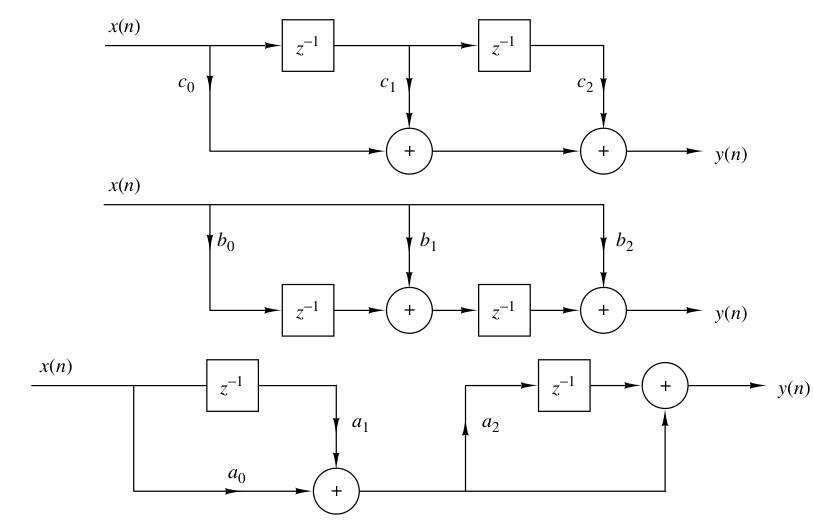
\includegraphics[width=14cm]{figures/fig52.png}
  \caption{Figure P52 from textbook}
    \label{fig:number52_fromText}
\end{figure}
\begin{enumerate}
\item Determine and sketch their impulse responses $h1 (n)$, $h2 (n)$, and $h3 (n)$.
\item Is it possible to choose the coefficients of these systems in such a way that: \center{$h_1 (n) = h_2 (n) = h_3 (n)$}
\end{enumerate}
\vspace{2em}
\hrule
\end{document}




